Ein Raspberry Pi, oft auch nur 'PI' genannt, ist ein vollwertiger Einplatinen-Computer. Das bedeutet, dass alle Komponenten, die in jedem Computer zu finden sind, auf einer einzigen Platine zu finden sind. Ausnahme dafür ist das Netzteil, welches meist aus einem 5 Volt USB C Kabel besteht. Als Betriebssystem wird das Linux-basierte System Raspberry Pi OS angeboten. Dieses besteht aus einem Desktop, einem Webbrowser, Einstellungen und Editoren für verschiedene Programmiersprachen. Der Mini-PC unterstützt jedoch auch andere Systeme, wie Raspberry Pi OS Lite, welches fast reines Linux ist. Dort findet man weder eine graphische Oberfläche noch vorinstallierte Apps.  

\begin{figure}[h t]
    \centering
    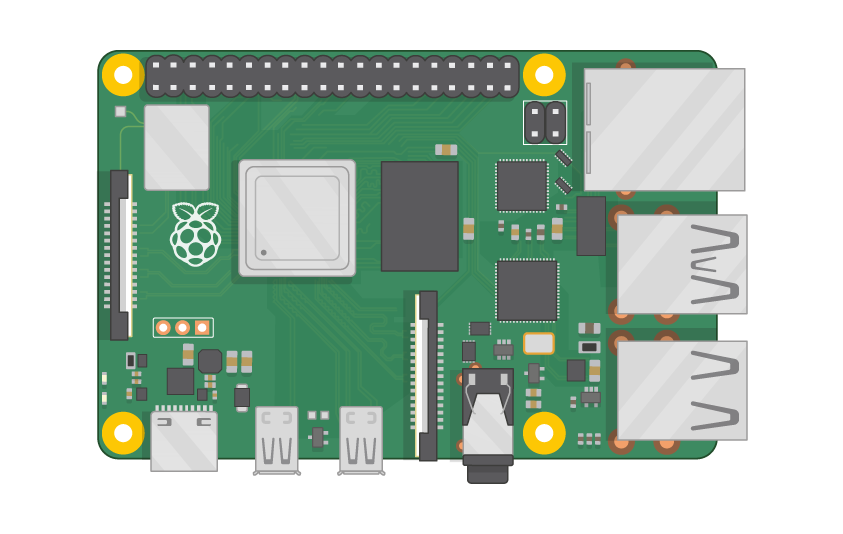
\includegraphics[scale=0.5]{pics/raspberry-pi.png}
    \caption{Aufbau eines Raspberry Pis}
    \label{fig:impl:RaspiAufbau}
  \end{figure}

  Da diese Mini-PCs in vielen Ausführungen und noch dazu relativ günstig zu haben sind, wurde für das Projekt ein Raspberry PI 4 ausgewählt. Dieser hat 4 GB RAM, eine Micro-SD-Karte mit einem vorkonfigurierten Image, einem Netzwerkanschluss und 4 USB-Steckplätze. Um die Zuverlässigkeit des Systems gewährleisten zu können, wurde ein Gehäuse von der Firma Flexsolution entwickelt, welches mit einem eingebauten Lüfter die Platinen kühlt. Des Weiteren wurde ein Modul installiert, welches einen Akku beinhaltet und den PI über eine 12 Volt-Leitung mit Strom versorgt. Dies ermöglicht eine Absicherung für Stromausfälle. Der Raspberry wurde in einem Schaltschrank montiert und an das Netzwerk angeschlossen.   

Solche Raspberrys werden in der Firma oft verwendet, da sie sich perfekt für die Flextask eignen. Sie sind günstig, leise, klein und verbrauchen kaum Strom. Sie können mit sogenannten GPIO-Pins mit Hardware interagieren und bieten eine Vielzahl an Möglichkeiten, Module anzuschließen.   